\documentclass{article}

\usepackage{courier}
\usepackage{graphicx} % Required for the inclusion of images
\usepackage{listings}
\usepackage{color}
\usepackage{amsmath}
\usepackage{subcaption}
\usepackage{enumitem}
\usepackage{float}
\usepackage[toc,page]{appendix}
\usepackage{dcolumn}
\usepackage{pdflscape}
\usepackage{hyperref}
\usepackage{framed}
\usepackage[english]{babel}
\usepackage{soul}
\usepackage{caption}
\captionsetup[figure]{labelformat=empty}%

\setlength\parindent{0pt} % Removes all indentation from paragraphs

\renewcommand{\labelenumi}{\alph{enumi}.} % Make numbering in the enumerate environment by letter rather than number (e.g. section 6)

\definecolor{dkgreen}{rgb}{0,0.6,0}
\definecolor{gray}{rgb}{0.5,0.5,0.5}
\definecolor{mauve}{rgb}{0.58,0,0.82}

\lstset{frame=tb,
  language=R,
  aboveskip=3mm,
  belowskip=3mm,
  showstringspaces=false,
  columns=flexible,
  basicstyle={\small\ttfamily},
  numbers=none,
  numberstyle=\tiny\color{gray},
  keywordstyle=\color{blue},
  commentstyle=\color{dkgreen},
  stringstyle=\color{mauve},
  breaklines=true,
  breakatwhitespace=true
  tabsize=3
}

%\usepackage[colorlinks]{hyperref}
\hypersetup{linkcolor=DarkRed}
\hypersetup{urlcolor=DarkBlue}
\usepackage{cleveref}

\title{Data Mining\\Homework Assignment \#8} % Title

\author{Dmytro Fishman, Anna Leontjeva and Jaak Vilo} % Author name

\begin{document}

\maketitle % Insert the title, author and date

\st{You are free to use any programming language you are comfortable with}. You will use Weka in this homework. Install Weka from \url{http://www.cs.waikato.ac.nz/~ml/weka}. Click around. Check the tutorial and other documentation here: \url{http://www.cs.waikato.ac.nz/ml/weka/documentation.htm}l.

\section*{Task 1}
We will start working with Weka using "Explorer" functionality. Now, load diabetes dataset, which comes with the weka. To do so, click on "Open file" and in default Weka directory find folder ``data'' with all the datasets inside. Use file diabetes.arff for this task. Open it and explore options of "Preprocess" tab. The description of diabetes dataset is here: \url{http://classes.soe.ucsc.edu/cmps142/Winter10/handouts/diabetes.arff}.
 
Next, choose "Classify" tab. Select J48 classifier ("choose" button and folder "trees"), run it, leaving the default parameters. Interpret the learned tree, plot it (right click on the model in the "Result list"). 

Characterize the TP, FP, TN, FN rates, accuracy, precision and recall obtained from this data. Make sure that you understand these metrics (intuitively and how they are calculated). What can be learned from this output?

\section*{Task 2}
Read more about ROC from Konstantin Tretyakov's blog post (\url{http://fouryears.eu/2011/10/12/roc-area-under-the-curve-explained/}) and the following Tom Fawcett's article: \url{http://tsam-fich.wdfiles.com/local--files/apuntes/ROCintro.pdf}. Plot the Receiving Operating Characteristic curve (ROC) for the model in Task 1 (right click on the model in "Result list" and "Visualize threshold curve"). Interpret it. 

\section*{Task 3}
Take a look at three examples below and answer the questions:
\begin{figure}[h!]
  \centering
      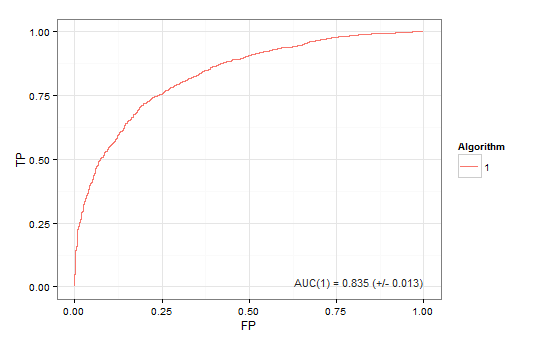
\includegraphics[width=0.8\textwidth]{plot1}
  \caption{What you can say about this ROC curve? How this classifier differs from a random guess. Pick one point on a curve and interpret it with toy example.}
\end{figure}
\begin{figure}[h!]
  \centering
      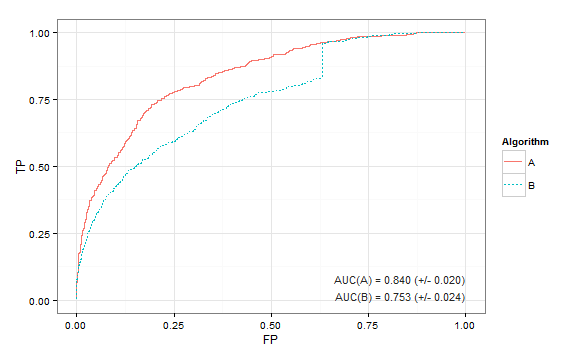
\includegraphics[width=0.8\textwidth]{plot2}
  \caption{Compare two ROC curves. Which one is a better model and why?}
\end{figure}
\begin{figure}[H]
  \centering
      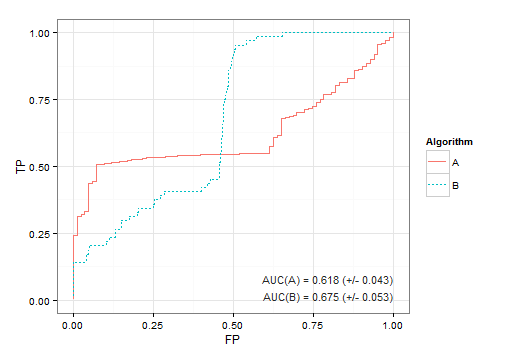
\includegraphics[width=0.8\textwidth]{plot3}
  \caption{Compare two ROC curves. When algorithm A would be preferred over algorithm B?}
\end{figure}

\section*{Task 4}
Calculate (on paper) confusion matrix, precision and recall for the given dataset under threshold of 0.5:
\begin{verbatim}
    True class  Prediction
1.   1           0.6
2.   1           0.8
3.   0           0.4	
4.   1           0.9
5.   0           0.7
6.   1           0.6
7.   1           1.0
8.   0           0.2
9.   0           0.4
10.  0           0.6
\end{verbatim}

Draw a ROC curve and calculate area under the curve (AUC).

\section*{Task 5}
Load data.arf to Weka, analyze it. Run the same J48 classifier as in the Task 1, study the results of the classification analysis. Draw ROC curve. What can you say about the results? Do measures agree? Explain the reason? Which measures should be preferred in this case?

\section*{Task 6}
Take the quiz: \url{https://www.proprofs.com/quiz-school/story.php?title=Njc3OTc3KPRO}
2 points will be given for grade "A" for the first trial and 1 point otherwise. 
\end{document}
